\documentclass[catalan,spanish,english]{exam}
\usepackage[T1]{fontenc}
\usepackage[latin9,utf8]{inputenc}
\setcounter{secnumdepth}{3}
\usepackage{babel}
\usepackage{amsfonts,amsmath,amssymb,amsthm}


%\usepackage[backend=bibtex]{biblatex}

% NEVER DO THIS AT HOME

\usepackage{epsfig,epstopdf}

\title{UIMP MASTER IN QUANTUM TECHNOLOGIES \\ FINAL EXAM COURSE 102776 \\ Quantum Computing: Theory and Practical Applications}

\author{Jara Juana Bermejo-Vega, Armando Pérez and Germán Sierra}

\date{February 6th, 2025}

\begin{document}

% COMENTO EN CLASE DE COMPU

\maketitle 

\selectlanguage{spanish}%
\global\long\def\abs#1{\left|#1\right|}%
\global\long\def\ket#1{\left|#1\right\rangle }%
\global\long\def\bra#1{\left\langle #1\right|}%
\global\long\def\half{\frac{1}{2}}%
\global\long\def\partder#1#2{\frac{\partial#1}{\partial#2}}%
\global\long\def\comm#1#2{\left[#1,#2\right]}%
\global\long\def\vp{\vec{p}}%
\global\long\def\vpp{\vec{p}'}%
\global\long\def\dt#1{\delta^{(3)}(#1)}%
\global\long\def\Tr#1{\textrm{Tr}\left\{  #1\right\}  }%
\global\long\def\Real#1{\mathrm{Re}\left\{  #1 \right\}  }%
\global\long\def\braket#1{\langle#1\rangle}%
\global\long\def\escp#1#2{\left\langle #1|#2\right\rangle }%
\global\long\def\elmma#1#2#3{\langle#1\mid#2\mid#3\rangle}%
\global\long\def\ketbra#1#2{|#1\rangle\langle#2|}%
\foreignlanguage{catalan}{}

\selectlanguage{english}%




To be returned to the course instructors by February 7th, 2025, 10:00 am (Madrid timezone) via the institutional UIMP email in the virtual campus. Ideally, send it as an attachment of a single email to all course instructors..

\paragraph{Problem 1 (Quantum Gates).}


Any state of the Block sphere can be constructed from the state $|0 \rangle$ as 
%
\begin{equation}
    | \psi( \theta, \phi ) \rangle  = 
R_z \left( \frac{ \pi}{2} + \phi \right) H   R_z \left( \theta \right) \, H \,  |0 \rangle, \quad R_z(\alpha) = e^{ - i \frac{\alpha}{2}   \sigma^z}  
\label{4-1}
\end{equation}
where  $H$ is the Hadamard gate. 

\begin{enumerate}
\item  Construct the unitary $U$ that implements the transformation 

$$
| \psi( \theta_2, \phi_2 ) \rangle  =  U  \, | \psi( \theta_1, \phi_1 \rangle) \rangle, \quad \forall  \; \theta_{1,2}, \phi_{1,2}
$$

\end{enumerate}


\paragraph{Problem 2 (Quantum Noise).}
Consider a qubit, whose states are described in the computational
basis $\{\ket 0,\ket 1\}$. Initially, the state of the qubit is given
by the operator density $\rho(0)=\ket 0\bra 0$. Assume that the qubit
interacts with the environment, and that this action can be described
by the Kraus operators $K_{1}=\sqrt{1-p}\,\,I_{2}$, $K_{2}=\sqrt{p}\,\,\sigma_{x}$,
where $I_{2}$ is the identity matrix, $\sigma_{x}$ the first Pauli
matrix, and $0\le p\le1$. Under the action of these operators, after
a time $t$ we obtain\foreignlanguage{spanish}{
\[
\rho(t)=\sum_{i=1}^{2}K_{i}\rho(0)K_{i}^{\dagger}
\]
}

\begin{enumerate}
    \item Calculate the entropy for the state $\rho(t)$. 
    \item Is it possible to
find a unitary operator $U(t)$ defined on the Hilbert space of the
qubit, such that $\rho(t)=U(t)\rho(0)U^{\dagger}(t)$? 

\item Now consider the alternative set of Kraus operators $K_{1}=a\,\sigma_{z}$,
$K_{2}=b\,\,\sigma_{x}$, with $a,b$ some real numbers. What kind
of restrictions can be placed on $a$ and $b$?
\end{enumerate}

ADDED SENTENCE.

ANOTHER SENTENCE.


\cite{skotiniotisQuantumMetrologyIsing2015}


\paragraph{Problem 3 (Quantum repetition code).} The 3-qubit quantum bit-flip code with stabilizer generators $\{ Z_1Z_2, Z_2Z_3\}$ can correct single-qubit Pauli $X$ errors. The 3-qubit quantum phase-flip code with stabilizer generators $\{ X_1X_2, X_2X_3\}$ can correct single-qubit Pauli $Z$ errors. Let $Y$ be the Pauli $Y$ gate, which fulfills the following conditions:
\begin{equation}
    Y=\textnormal{i}XZ, \qquad  Y=S X S^\dagger, \quad S=
    \begin{pmatrix}
        1 & 0 \\ 
        0 & \textnormal{i}
    \end{pmatrix}.
\end{equation}
In short, $Y$ is Hermitian and  identical to $X$ via the unitary change of basis $S$. Below, we are asked to design quantum error correcting codes   for single-qubit Pauli noise channels of the form  $\mathcal{E}_U(\rho)= p \rho + (1-p) U \rho U $, where a Pauli error  $U\in \{I, X, Y, Z\}$ occurs with some probability $p>0$.
\begin{enumerate}
    \item (A different phase-flip code). Show that the repetition code with stabilizer operators $\{ Y_1Y_2, Y_2Y_3\}$ can detect and correct single-qubit Pauli $Z$ errors of the form  $\mathcal{E}_Z(\rho)= p \rho + (1-p) Z \rho Z $. Describe a quantum circuit for measuring the parity operator $Y_1Y_2$ of this code.
    \item   (A quantum ``$Y$-flip'' code).  An experimentalist team has built a faulty quantum computer where qubits are affected by a noise process $\mathcal{E}_Y(\rho)= p \rho + (1-p) Y \rho Y $. Argue that the quantum ``$Y$-flip'' code with stabilizer generators $\{ Z_1Z_2, Z_2Z_3\}$ can detect and correct single-qubit Pauli $Y$ errors.
    \item (A different Bacon-Shor code). Concatenate the repetition code $\{ Y_1Y_2, Y_2Y_3\}$ with the  bit-flip code $\{ Z_1Z_2, Z_2Z_3\}$ to define a modified 9-qubit Bacon-Shor code with stabilizer generators 
  $Z_1 Z_2$, $Z_2Z_3$, $Z_4 Z_5$, $Z_5Z_6$, $Z_7 Z_8$, $Z_8Z_9$, $Y_1Y_2Y_3Y_4Y_5Y_6$, and $Y_4Y_5Y_6 Y_7 Y_8 Y_9$. Argue that this code can correct all single-qubit errors of arbitrary form. (Recall that $\{I, X, Y, Z\}$, the four Pauli matrices, define an operator basis for a single qubit, i.e., any Kraus operator $K$ associated to a single-qubit error can be written as a linear combination $K= a_I I + a_X X + a_Y Y + a_Z Z$ with complex coefficients.)
    %\item  ($Z$ errors in the bit-flip code). Convince yourself that the 3-qubit quantum bit-flip code cannot correct phase-flip errors. To this end, show that measuring the parity operators $Z_1 Z_2$, $Z_2 Z_3$ cannot detect whether a $Z$ error happened. (You may do so by using the simple quantum error correction conditions for stabilizer codes, or by evaluating the action of the errors and measurements on codewords.)
    \item The quantum experimentalists team reports that some mysterious damage has occurred to their  quantum computer. We observe that now there is a faulty qubit that is affected by both $X$ and $Y$ errors with even probability: $\mathcal{E}_{X,Y}(\rho)= p \rho + (1-p)/2 (X\rho X + Y \rho Y)$, with $p>0$. On the other hand, $Z$-errors never occur. Answer: can we use the ``Y-flip code'' to correct these errors? Is it possible to  distinguish $X$ and $Y$ errors  by measuring the parity operators  $Z_1 Z_2$, $Z_2 Z_3$?
\end{enumerate}
Hints: The stabilizer formalism for quantum codes that we studied in the lectures is quite handy in situations where calculations with wavefunctions become complex. Calculations with stabilizer codes can also  be  simplified by performing a Clifford change of basis. For instance, in the course, we derived the properties of the phase-flip code by mapping it to a bit-flip code in the Hadamard basis. 

\paragraph{Problem 4. Gate teleportation with graph states.}
The brickwork state is a universal resource for measurement-based quantum computation with applications for blind quantum computing. It is a 2D graph state, with the geometry given in the figure below. Therein, blue balls represent qubits prepared in the $\ket{+}=(\ket{0}+\ket{1})/\sqrt{2}$ state. Edges in the graph represent $CZ=\mathrm{diag}(1,1,1,-1)$ gates that are used to create entanglement accross qubits. The qubits with the label ``0" are measured with a zero-angle in the X-Y plane: i.e., single-qubit $X$ measurements are performed in all of them.
 \begin{figure}[ht] 
 \centering
   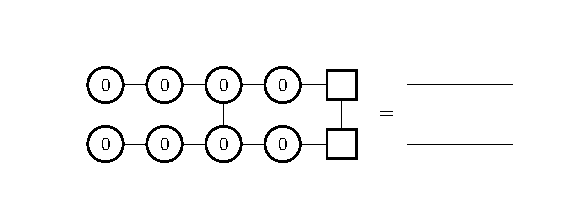
\includegraphics{f4}
 \label{Fig:identity}
 \end{figure}
\begin{enumerate}
    \item Prove that this measurement pattern implements a two-qubit identity gate modulo some Pauli operation: i.e., it teleports a two-qubit state from left to right and adding some byproduct Pauli operation to it.
    \item Imagine the teleported state is measured in the standard basis. Show that the action of a byproduct  prior to the measurement Pauli operation is to permute the outcomes in a predictable deterministic way. Discuss: does this jeopardize the outcome of a quantum computation?
\end{enumerate}

\cite{bermejo-vegaNormalizerCircuitsGottesmanKnill2015}

\cite{raussendorfContextualityWignerfunctionNegativity2017a}\cite{manzanoShortIntroductionLindblad2020}


\bibliographystyle{naturemag}

\bibliography{database.bib}


\end{document}

